\chapter{提案モデル}

\begin{figure}[b]
\begin{center}
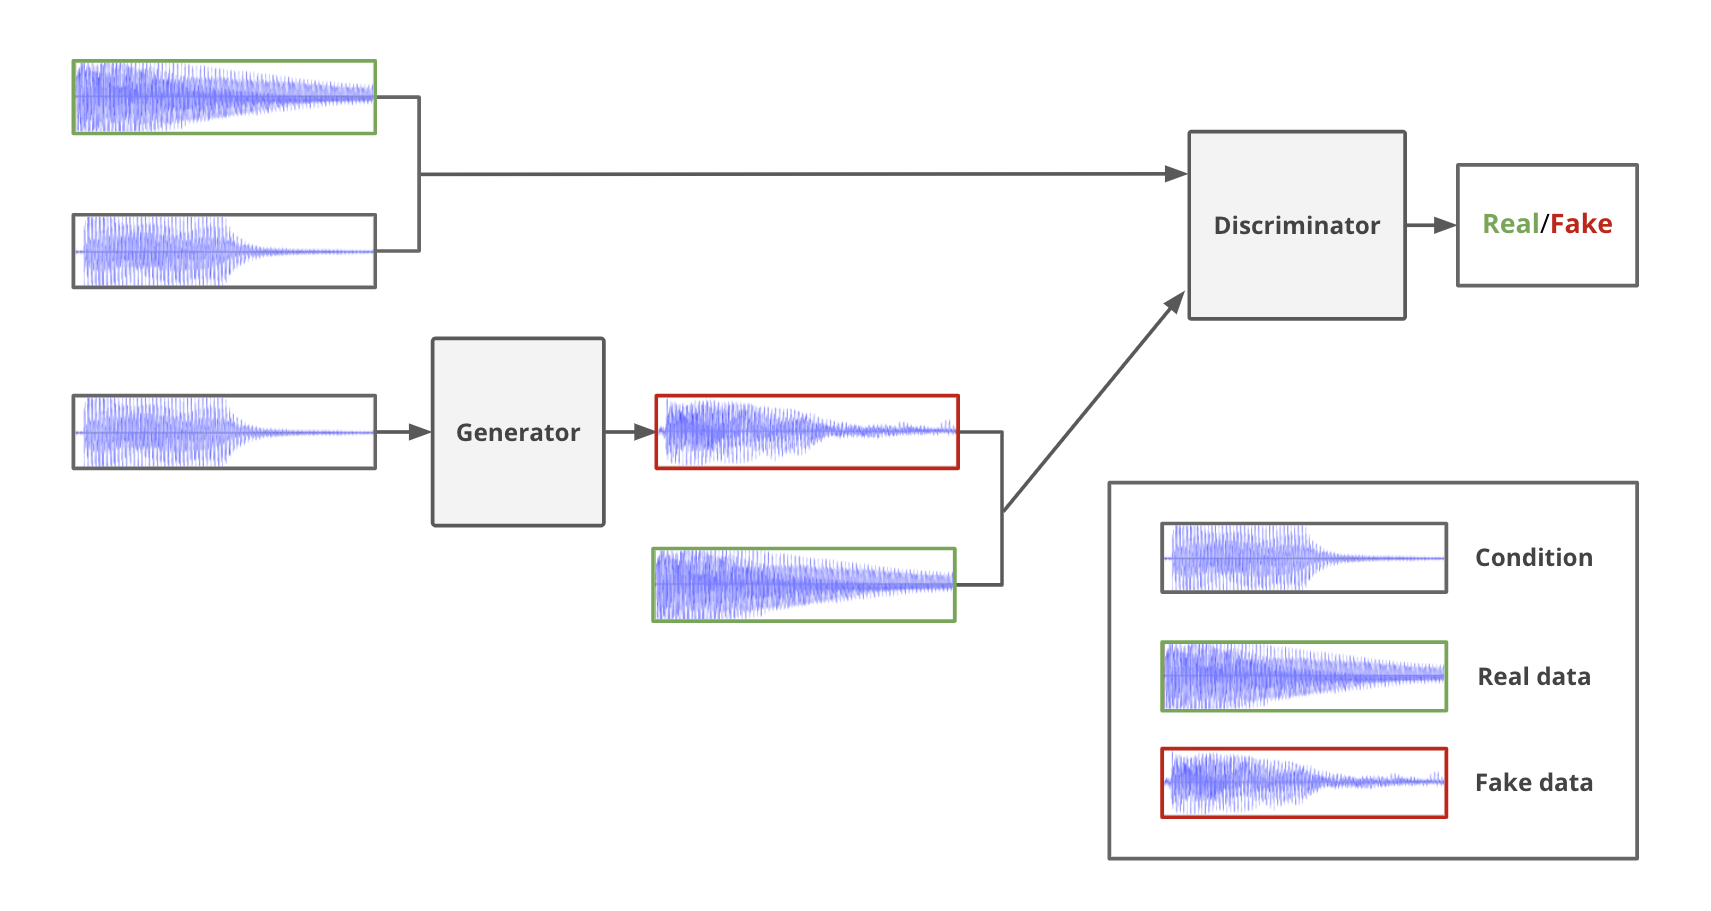
\includegraphics[width=\hsize]{figure/pr_model.png}
\caption{提案モデル}
\label{fig:pr_model}
\end{center}
\end{figure}

本研究では、図\ref{fig:pr_model}のようなPix2pixを元に作成したモデルを提案する~\cite{pix2pix}。このモデルでは、生成モデルと識別のいずれにも条件として変換元の音を入力している。また、決定論的に音を生成するために、生成モデルの入力にノイズを使用していない。

\section{前処理}

本研究では、44100~Hzのサンプリング周波数でサンプリングした1秒の音波をそのまま使用する。また、量子化ビット数を16ビット、チャンネル数を1として固定しているため、44100の長さを持つ16ビット整数の一次元配列として音を扱う。

\section{ネットワーク構造}

図\ref{fig:pr_gen}及び図\ref{fig:pr_dis}に生成モデルと識別モデルのネットワーク構造をそれぞれ示す。まず、図にある灰色の箱は複数チャンネルの特徴量マップである。箱の上側にチャンネル数を示し、箱の左側に特徴量マップとなる一次元配列の長さを示している。そして、ネットワーク構造の下にはそれぞれの矢印の操作を示している。ConvolutionとDeconvolutionについては~(カーネルサイズ、パディング数、ストライド幅)~としてそれぞれの値を示し、LeakeyReLUについては負の実数の定義域での一次関数の傾きの値を示す。

\subsection{生成モデル}

\begin{figure}[t]
\begin{center}
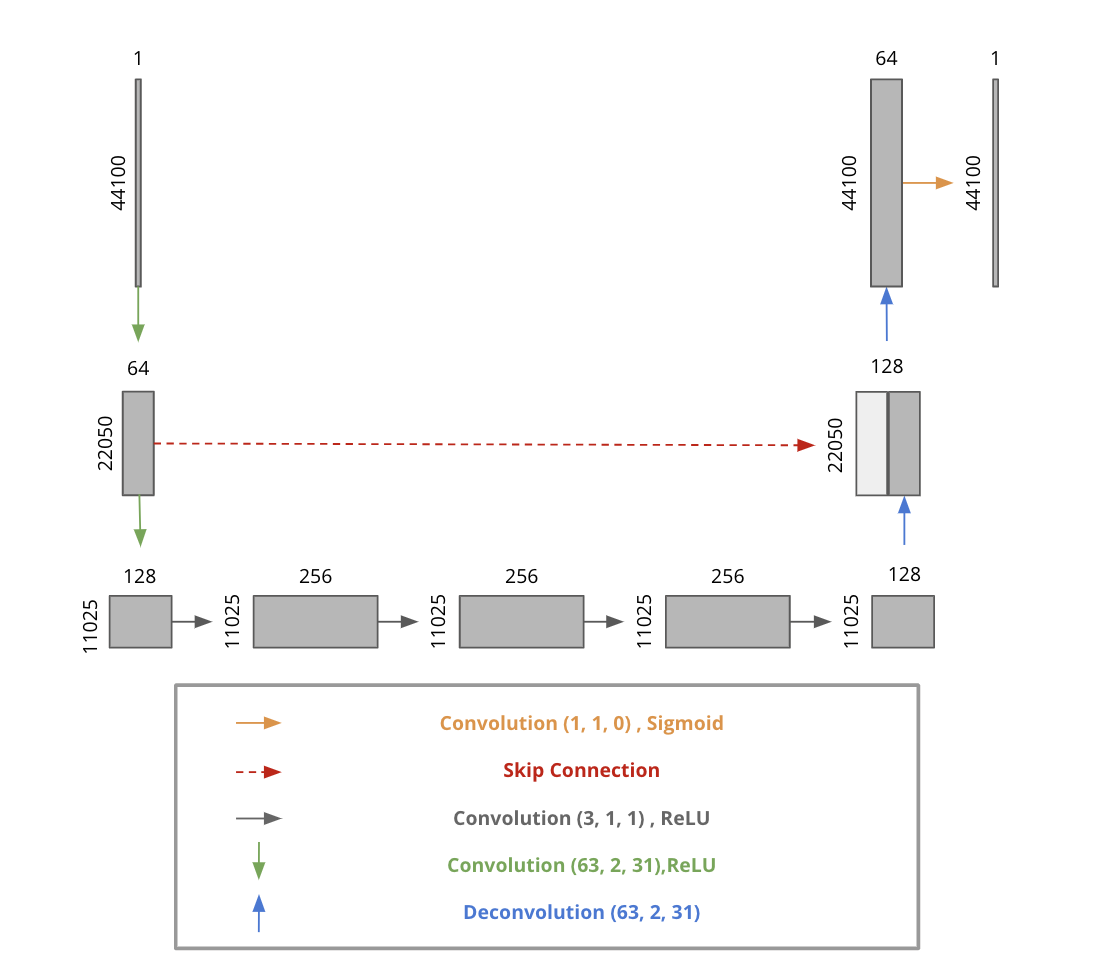
\includegraphics[width=0.8\hsize]{figure/pr_generator.png}
\caption{生成モデル、図は文献~\cite{u-net}のFigure~1を参考に作成。}
\label{fig:pr_gen}
\end{center}
\end{figure}

本研究では、生成モデルに図\ref{fig:pr_gen}のような1つのスキップコネクションを持つEncoder-Decoder型のネットワークを用いた。それぞれのパラメータは図\ref{fig:pr_gen}に示す。

\subsection{識別モデル}

\begin{figure}[t]
\begin{center}
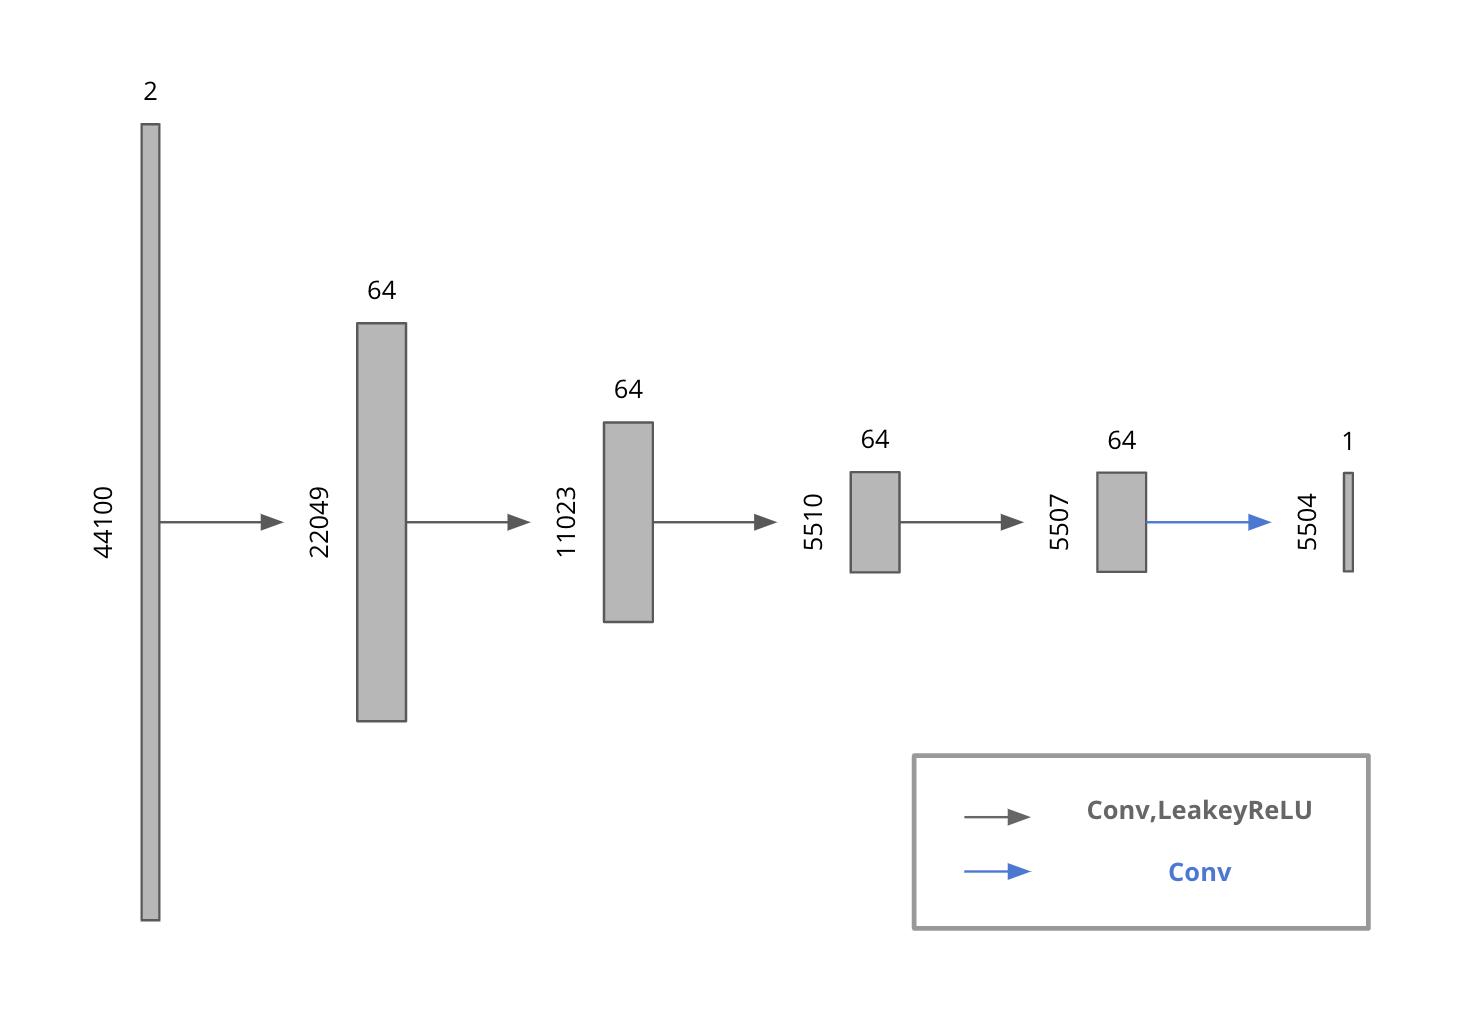
\includegraphics[width=0.8\hsize]{figure/pr_discriminator.png}
\caption{識別モデル、図は文献~\cite{u-net}のFigure~1を参考に作成。}
\label{fig:pr_dis}
\end{center}
\end{figure}

本研究では、識別モデルに\ref{fig:pr_dis}のようなCNNを用いた。それぞれのパラメータは図\ref{fig:pr_dis}に示す。

\chapter{実験}

本章では、実験で用いるデータセットや実験方法などについて説明した後、実験結果の考察を行う。

\section{データセット}

\begin{figure}[t]
\begin{center}
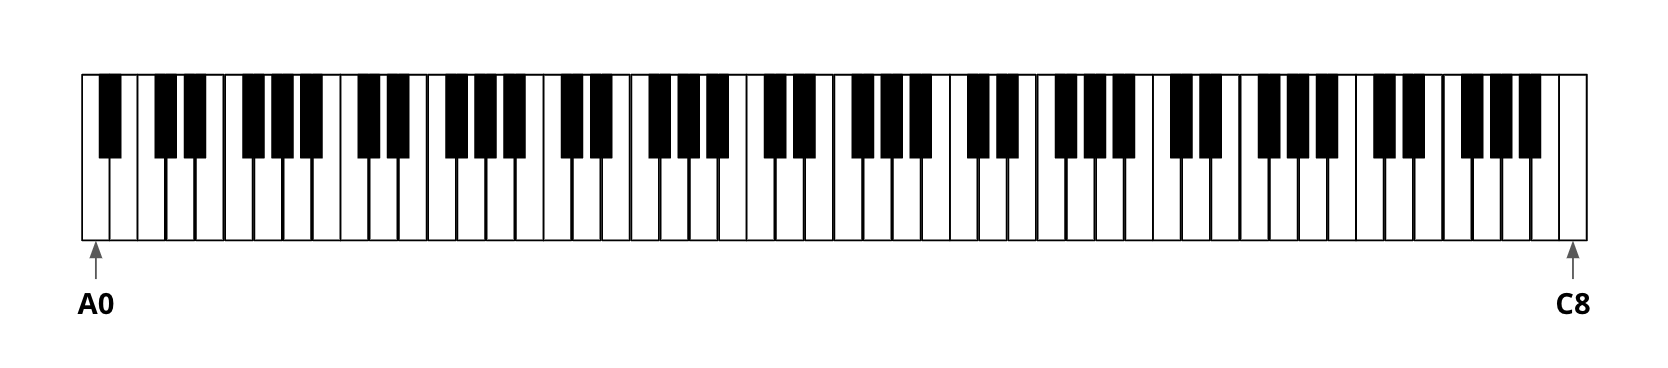
\includegraphics[width=\hsize]{figure/piano.png}
\caption{88鍵のピアノの鍵盤}
\label{fig:piano}
\end{center}
\end{figure}

1秒のギターとハープの音の88組をデータセットとして用意した。また、データ形式としては非圧縮形式で波形を保持するWAV形式を採用した。88音としてはA0$\sim$C8の半音を全て選んだが、これらは図\ref{fig:piano}のような一般的な88鍵のピアノで用いられる音である。

\section{評価方法}

生成した音は音波の波形の観察と音の聴き取りにより評価した。また、以降で示す波形の図は三つの音波を並べたものであり、変換元のギター、生成モデルの出力、変換先のハープ、の順で並べている。そして、生成モデルの出力が音の高さ及び音の大きさを保持したまま変換先のハープの音の音色に変換できているかという観点から評価を行った。

\section{実験時の工夫}

%位相をずらす
%バッチサイズの調整?
実験時には学習データの振幅を無作為化する工夫を行った。具体的には、学習データの振幅を$0.3\sim1.0$倍した。また、学習前に乱数のシードを固定した後に一様乱数により生成している。この工夫によりデータを拡張することができ、88音と小さいサイズのデータセットへの過学習を防ぐことができていると期待した。

\section{実験方法}

提案モデルを用いて十分に音色が異なると考えられるギターからハープへの音の変換の実験を行った。学習と評価の際のパラメータは付録\ref{sec:appendix}の\ref{sec:appendix_params}節に示す。また、本研究で行うモデルの学習にはAdamを用いた。

\subsection{生成モデルの表現力の評価}

まず、本手法のニューラルネットワークの生成モデルが十分な表現力を有し、識別モデルが正確に判定を行うことができるかを確認するため、学習データと評価データにそれぞれ同じ88音のデータセットを用いて実験を行う。

\subsection{生成モデルの汎化能力の評価}

一般に、単音の音色変換において任意の高さと大きさの音を学習データとして用意するのは不可能である。従って、未知のデータも適切に処理できるニューラルネットワークを構築する必要がある。このような、未知のデータを適切に処理できる能力のことを汎化能力と呼ぶ。

本手法のニューラルネットワークが未知のデータも適切に処理できるか調べるため、88音のうち3/4を学習データ、1/4を評価データとする4分割交差検定を行う。この際のデータセットの分割方法は付録\ref{sec:appendix}の\ref{sec:appendix_split}節に示す。

\section{実験結果}

本節では、実験結果及びその考察をまとめる。実験結果に記載する画像については三つの波形を上から並べており、上から順に元のギターの波形,変換後の波形,ハープの波形となっている。

%楽音→音の高さ→音の音色で達成度をまずは書くと良い

\subsection{生成モデルの表現力の評価}
\label{sec:expression}
%lossの図

\begin{figure}[t]
\begin{center}
\begin{minipage}{0.48\hsize}
\begin{center}
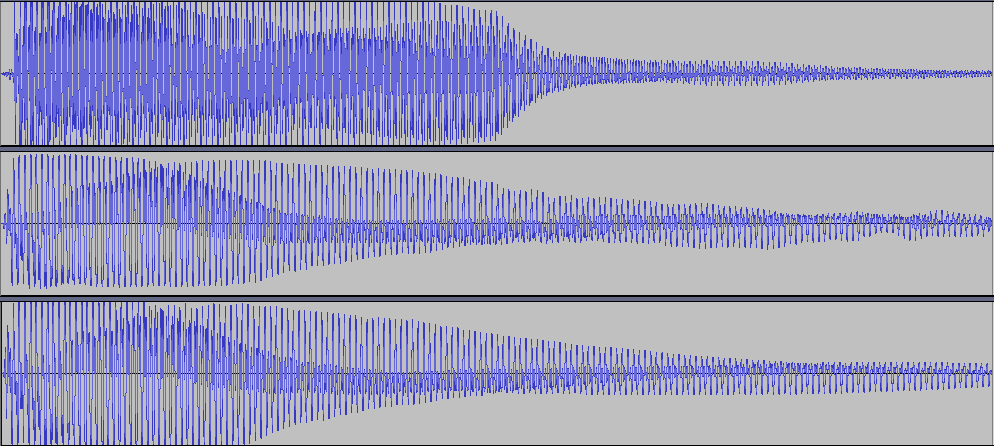
\includegraphics[width=0.9\hsize]{figure/88_88/f3.png}
\caption{F3の0.800秒から1.000秒までの音波}
\label{fig:88_88_good1}
\end{center}
\end{minipage}
\begin{minipage}{0.48\hsize}
\begin{center}
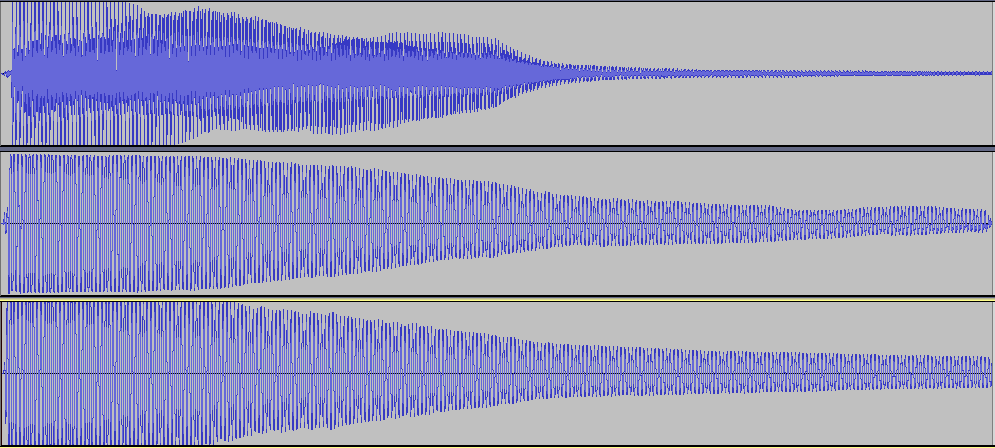
\includegraphics[width=0.9\hsize]{figure/88_88/c4.png}
\caption{C4の0.200秒から0.300秒までの音波}
\label{fig:88_88_good2}
\end{center}
\end{minipage}
\end{center}
\end{figure}


まず、F2からG6$\sharp$の音は耳で聴いても波形を見ても図\ref{fig:88_88_good1}のように正確にハープの音を表現することができていた。特にC4からD5$\sharp$の音は図\ref{fig:88_88_good2}のように上音の音が少ないために綺麗なハープの音を生成することができていた。他の音についても下記に挙げた改善点はあるものの基音の部分は表現することができていた。以下では、ハープの音を生成において困難であった点を列挙する。


\subsubsection{音波の振幅}

\begin{figure}[t]
\begin{center}
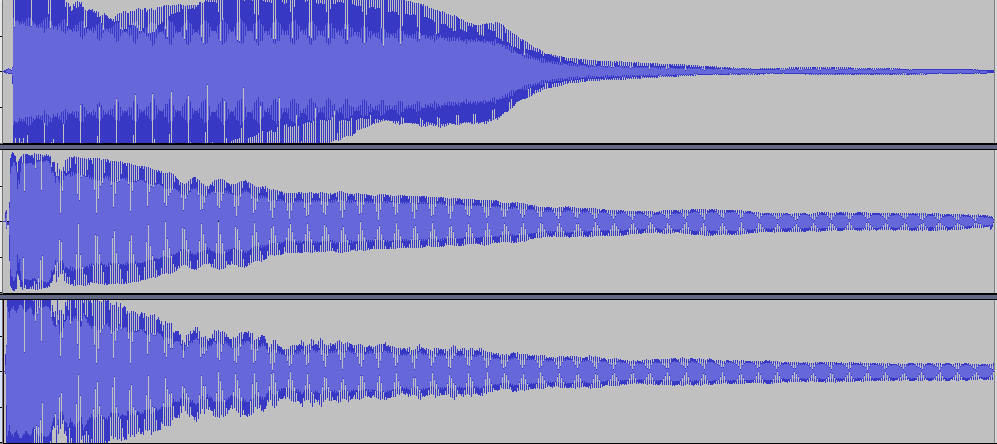
\includegraphics[width=0.7\hsize]{figure/88_88/c5.png}
\caption{C5の0.000秒から1.000秒までの音波}
\label{fig:88_88_amp}
\end{center}
\end{figure}

図\ref{fig:88_88_amp}の波形の前半のように、生成された波形の振幅が小さいという問題が発生した。これにより、減衰していく部分の表現が難しい場合があった。原因は、振幅をランダムに小さくしたためであると考えられ、学習の初段階では振幅を固定するなどの工夫する必要があると思われる。
    
\subsubsection{音の鳴り出しの遅延}

\begin{figure}[t]
\begin{center}
\begin{minipage}{0.48\hsize}
\begin{center}
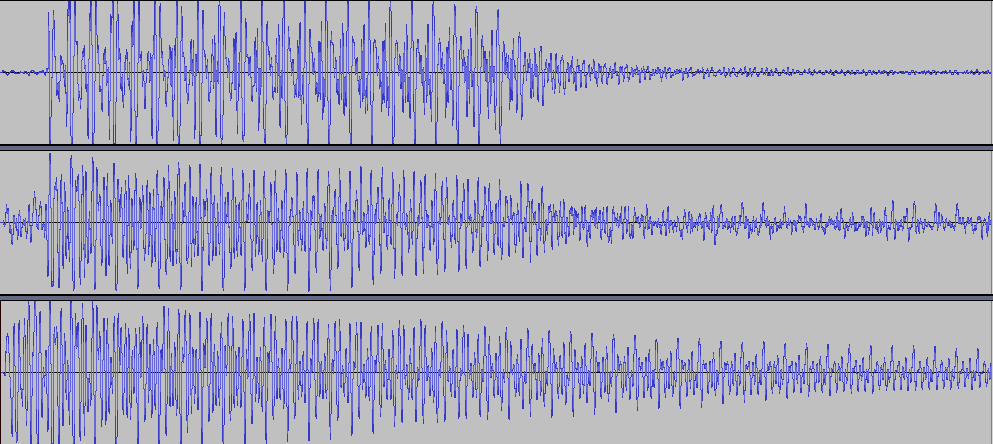
\includegraphics[width=0.9\hsize]{figure/88_88/f1s.png}
\caption{F1$\sharp$の0.000秒から1.000秒までの音波}
\label{fig:88_88_lag1}
\end{center}
\end{minipage}
\begin{minipage}{0.48\hsize}
\begin{center}
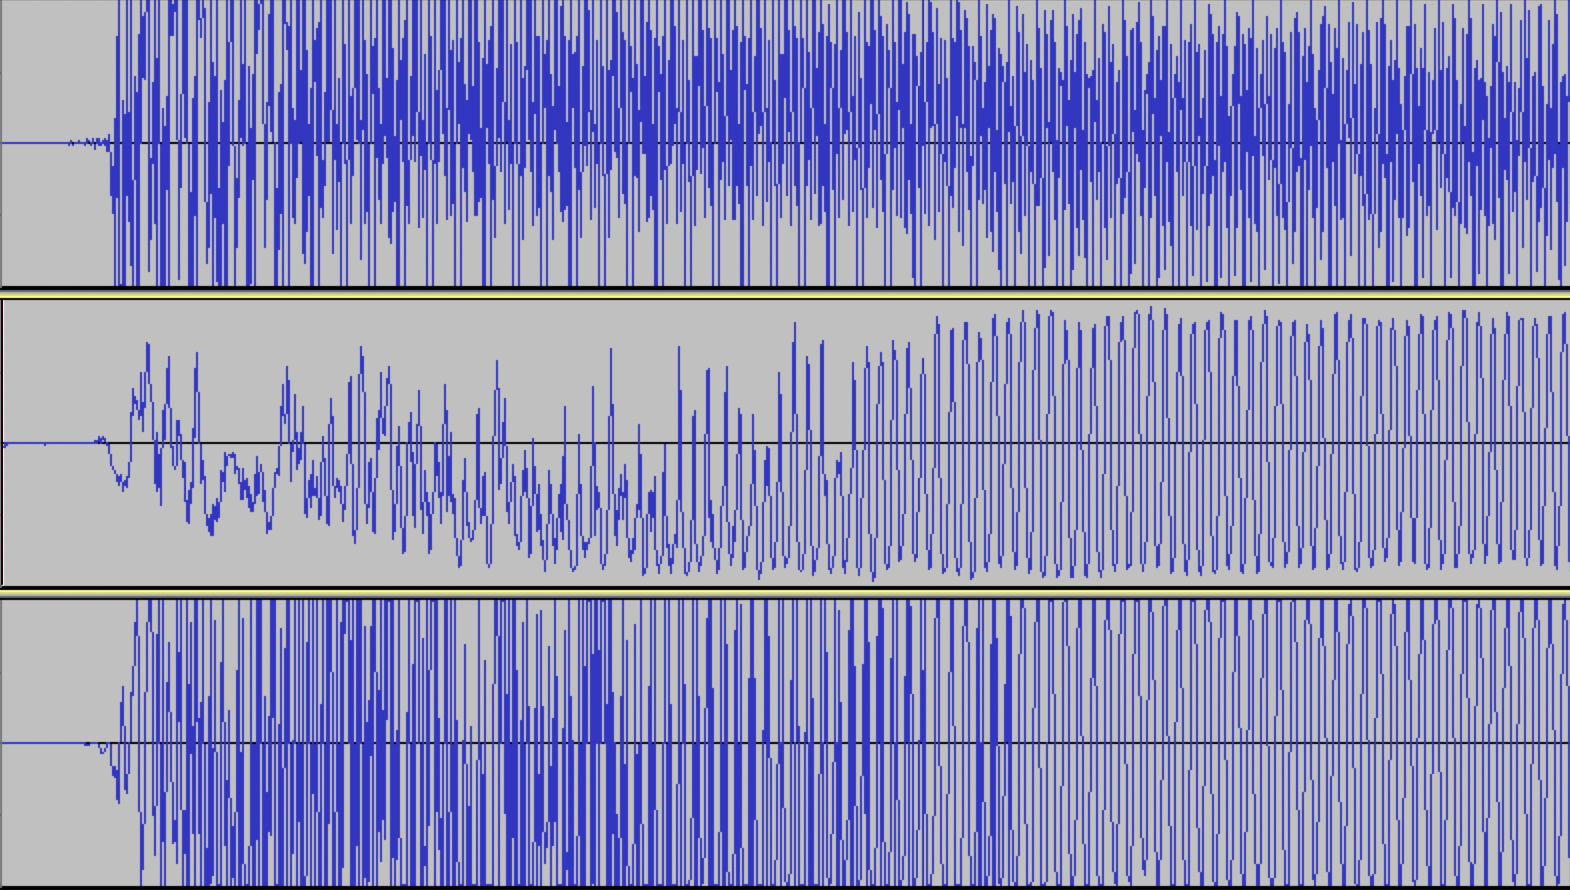
\includegraphics[width=0.9\hsize]{figure/88_88_det/a7_0_0030.png}
\caption{A7の0.000秒から0.030秒までの音波}
\label{fig:88_88_lag2}
\end{center}
\end{minipage}
\end{center}
\end{figure}

ギターとハープは弦楽器なので鳴り出すまでに遅延がある。特に、今回用いたデータセットでは図\ref{fig:88_88_lag1}のようにギターの音に遅延がある場合や図\ref{fig:88_88_lag2}のように周期的な音になるまでに遅延がある場合、その部分を学習することが難しかった。

\subsubsection{音波の滑らかさ}

\begin{figure}[t]
\begin{center}
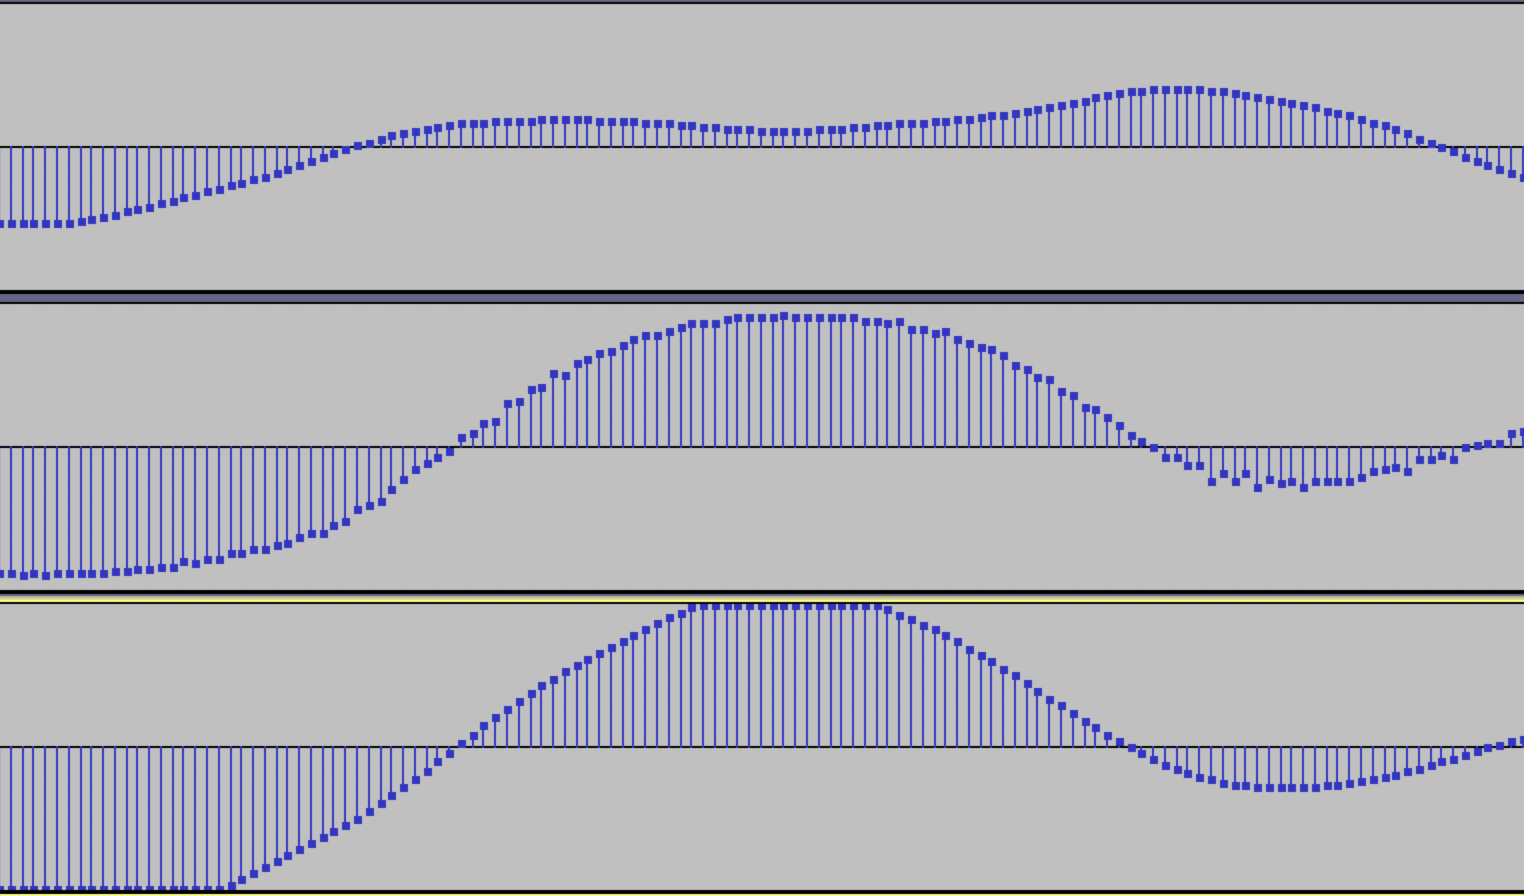
\includegraphics[width=0.7\hsize]{figure/88_88_det/d2s_0100_0103.png}
\caption{D2$\sharp$の0.100秒から0.103秒までの音波}
\label{fig:88_88_smooth}
\end{center}
\end{figure}

%滑らかさの表現
図\ref{fig:88_88_smooth}の上から2番目の波形と3番目の波形を比較すると、生成された波には滑らかさがないことがわかる。人間の耳にはこの滑らかでない音波の部分はノイズまじりの音として聞こえるので、この波を滑らかにするための工夫が必要であると考えられる。

\subsubsection{音波の振動の減衰}

\begin{figure}[t]
\begin{center}
\begin{minipage}{0.48\hsize}
\begin{center}
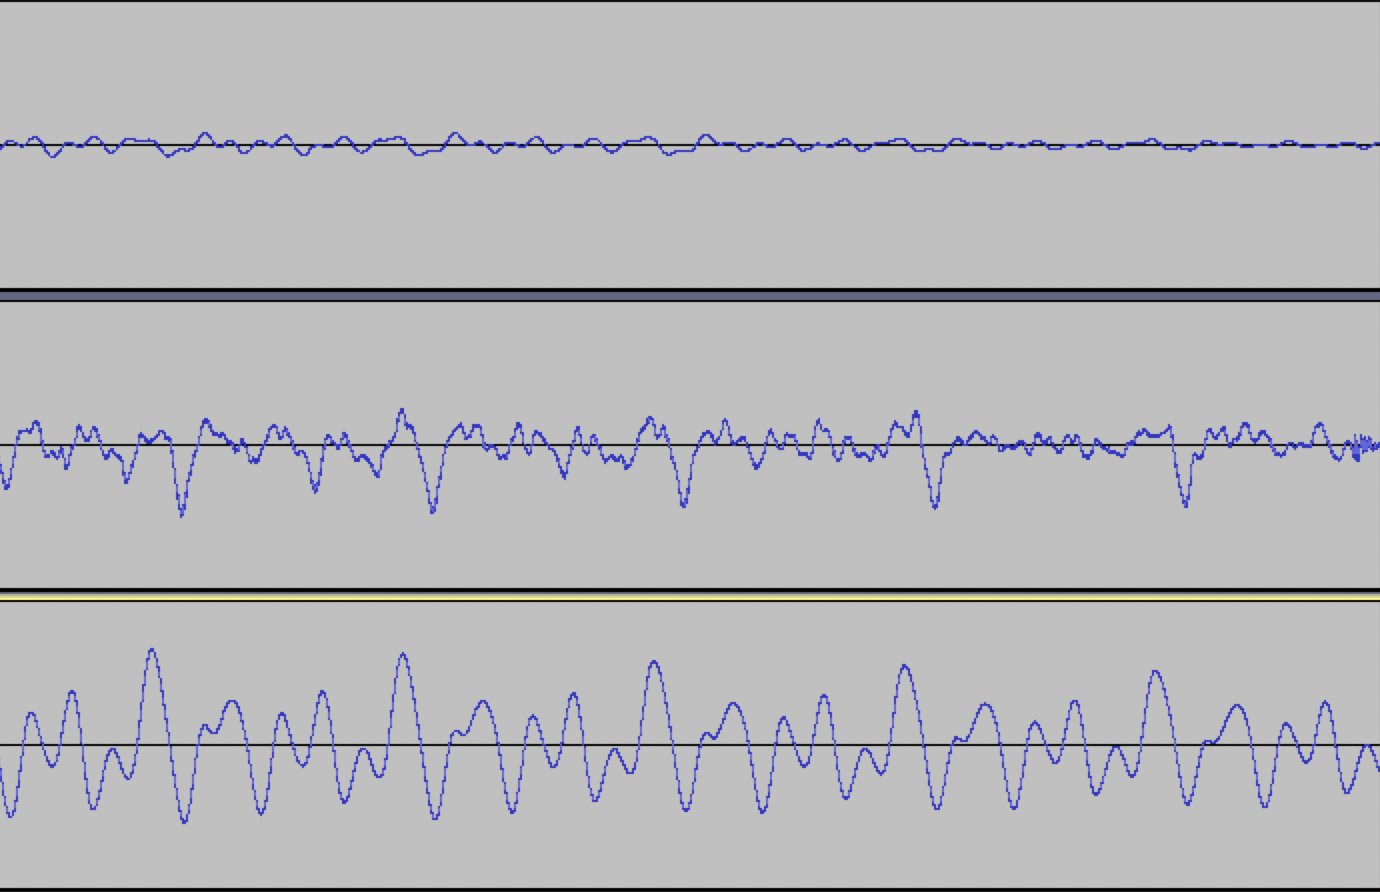
\includegraphics[width=0.9\hsize]{figure/88_88_det/a0_0800_1000.png}
\caption{A0の0.800秒から1.000秒までの音波}
\label{fig:88_88_reduce1}
\end{center}
\end{minipage}
\begin{minipage}{0.48\hsize}
\begin{center}
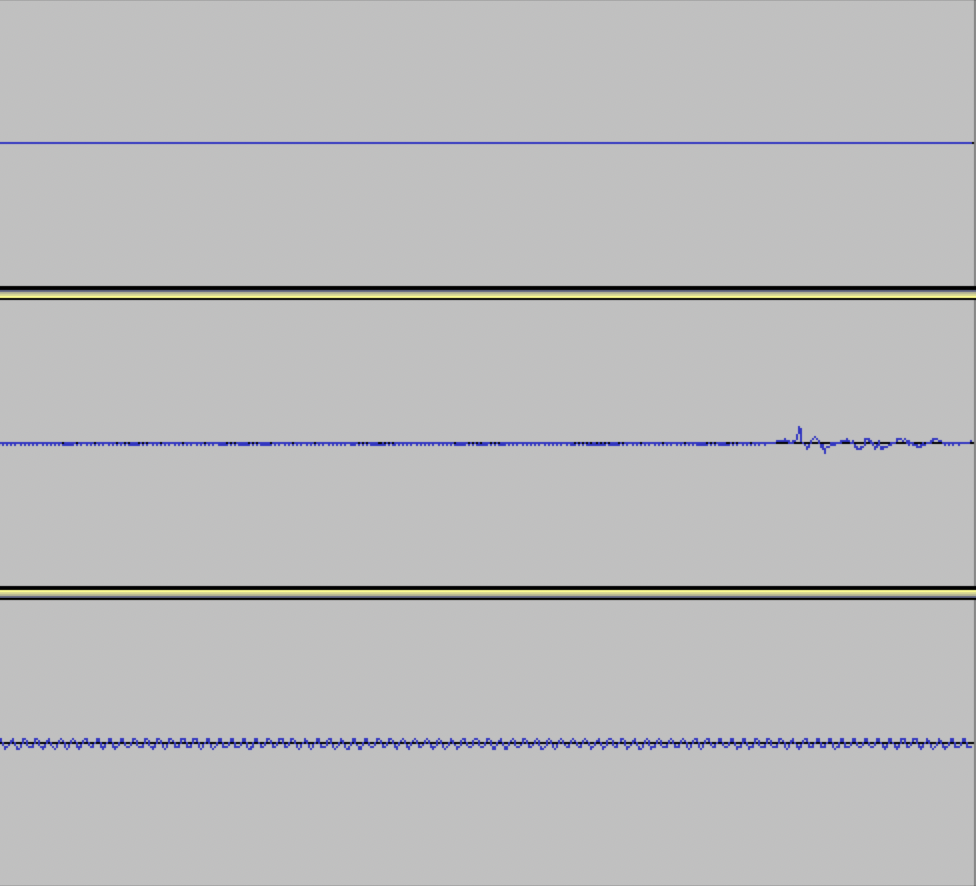
\includegraphics[width=0.9\hsize]{figure/88_88_det/b7_0980_1000.png}
\caption{B7の0.980秒から1.000秒までの音波}
\label{fig:88_88_reduce2}
\end{center}
\end{minipage}
\end{center}
\end{figure}

音波の振動の減衰が全く表現できていない音波があった。具体的には、A0,A0$\sharp$,B0,C1,C1$\sharp$,D1,D1$\sharp$,E1,\\
F1,F1$\sharp$,G1,G1$\sharp$D2,D2$\sharp$,E2,A6,A6$\sharp$,B6,C7,C7$\sharp$,D7,D7$\sharp$,F7,F7$\sharp$,G7,G7$\sharp$,A7,A7$\sharp$,B7,C8の音である。また、これ以外の音についても減衰が一部表現できていないものはあった。

これらの音のうち、E2以下の低音域の場合は図\ref{fig:88_88_reduce1}のようにハープとは全く異なる波形で減衰し、A6以上の高音域の場合は図\ref{fig:88_88_reduce2}のようにほとんど振動が見られなかった。原因としては、微小な振動をニューラルネットワークが学習するのが難しいことと今回のデータセットではギターの方がハープよりも音の鳴る時間が短かったことが挙げられる。

\subsubsection{安定したデータセットの作成}

\begin{figure}[t]
\begin{center}
\begin{minipage}{0.48\hsize}
\begin{center}
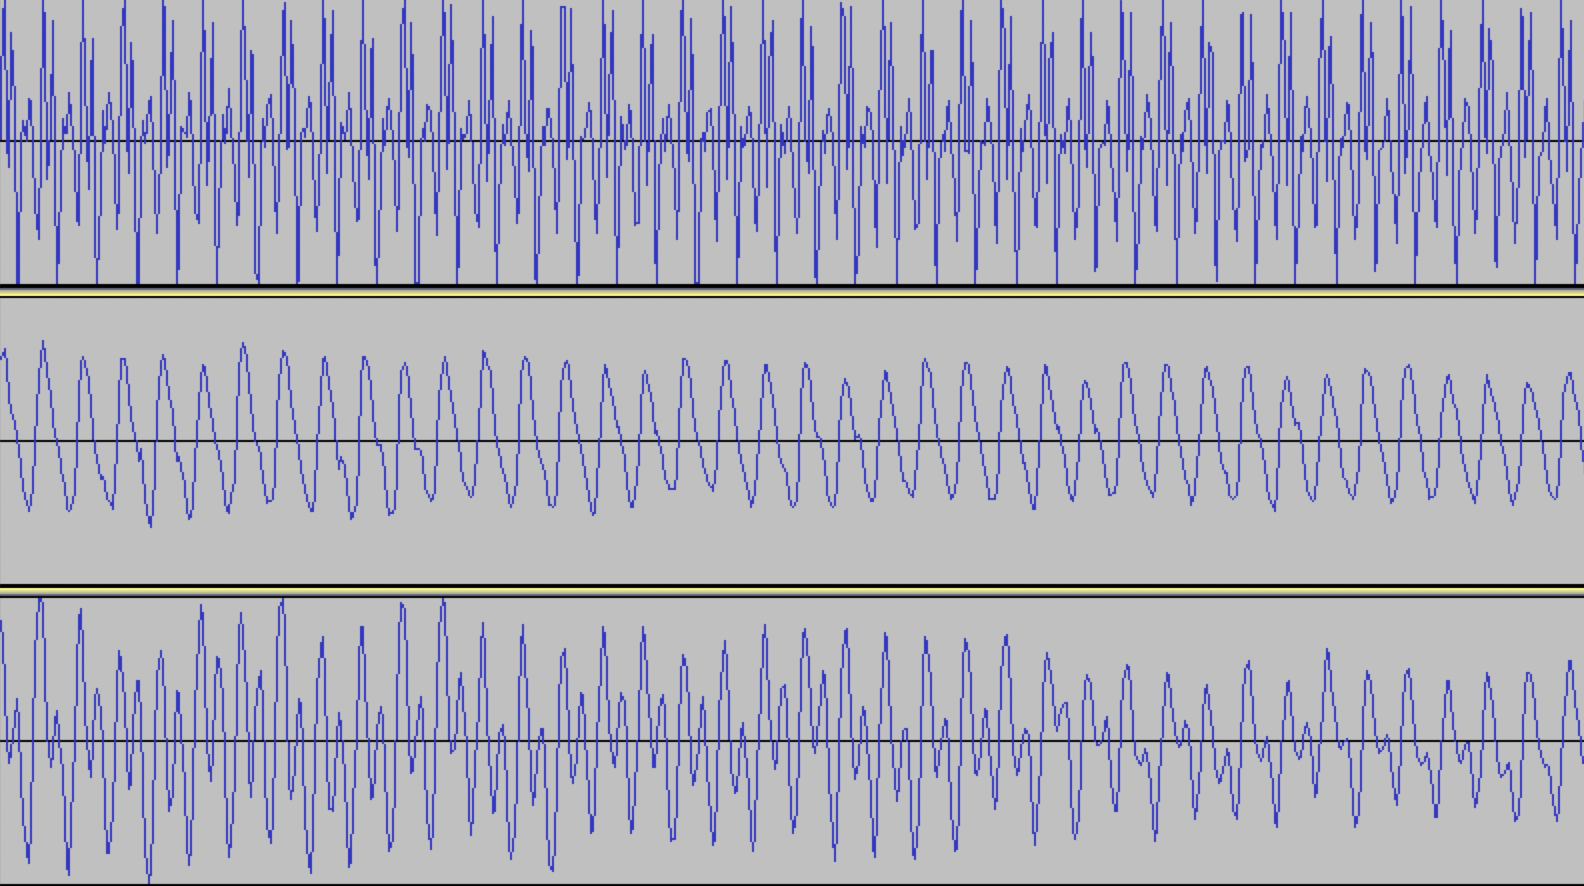
\includegraphics[width=0.9\hsize]{figure/88_88_det/e7_0550_0700.png}
\caption{E7の0.055秒から0.070秒までの音波}
\label{fig:88_88_bad1}
\end{center}
\end{minipage}
\begin{minipage}{0.48\hsize}
\begin{center}
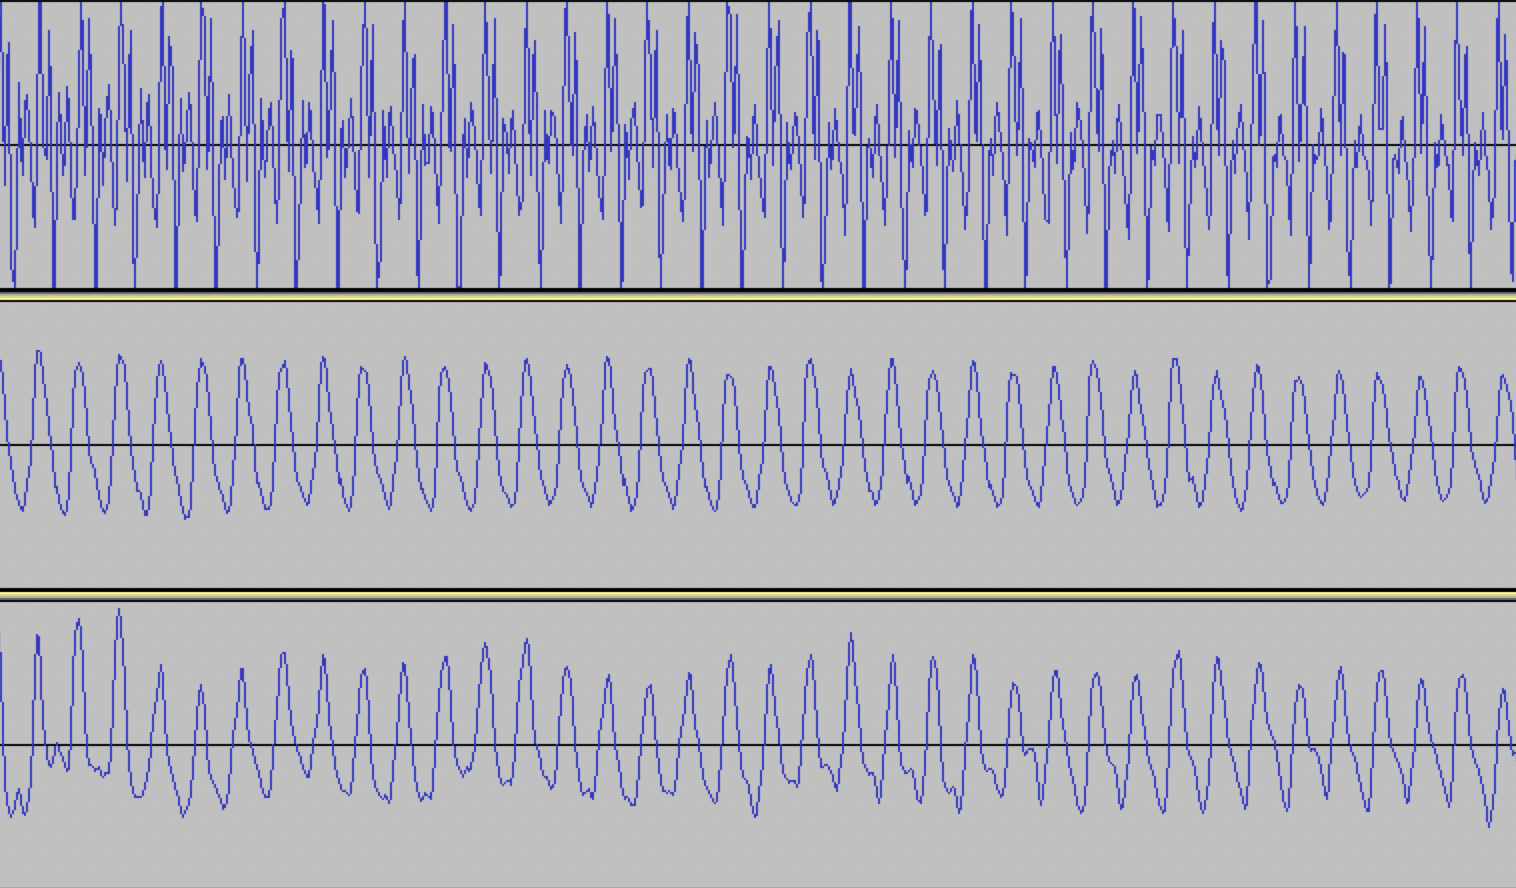
\includegraphics[width=0.9\hsize]{figure/88_88_det/d7s_0550_0700.png}
\caption{D7$\sharp$の0.055秒から0.070秒までの音波}
\label{fig:88_88_bad2}
\end{center}
\end{minipage}
\end{center}
\end{figure}

E7の音については、図\ref{fig:88_88_bad1}のように上記に挙げた以外の部分で波が表現できていなかったが、ハープのデータセットの音波の振動の振幅が安定していないために、ニューラルネットワークによる学習が難しかったと考えられる。

また、E7の半音下の音であるD7$\sharp$でも図\ref{fig:88_88_bad2}のようにハープのデータセットの音波の振動の振幅は安定しておらず、特に高音は安定した振幅のデータセットを生成することが難しいと考えられる。

\subsection{生成モデルの汎化能力}

まず、音の高さは変換前後で変わってないものが多く期待通りの結果となった。しかし、音の音色は元のギターの音色とは異なるもののハープとも異なる音色となり、\ref{sec:expression}節における課題も解決することはできなかった。以下では、生成されたハープの音について波形を元に考察を行う。

%学習の際のlossの図

\subsubsection{音波の単純さ}

\begin{figure}[t]
\begin{center}
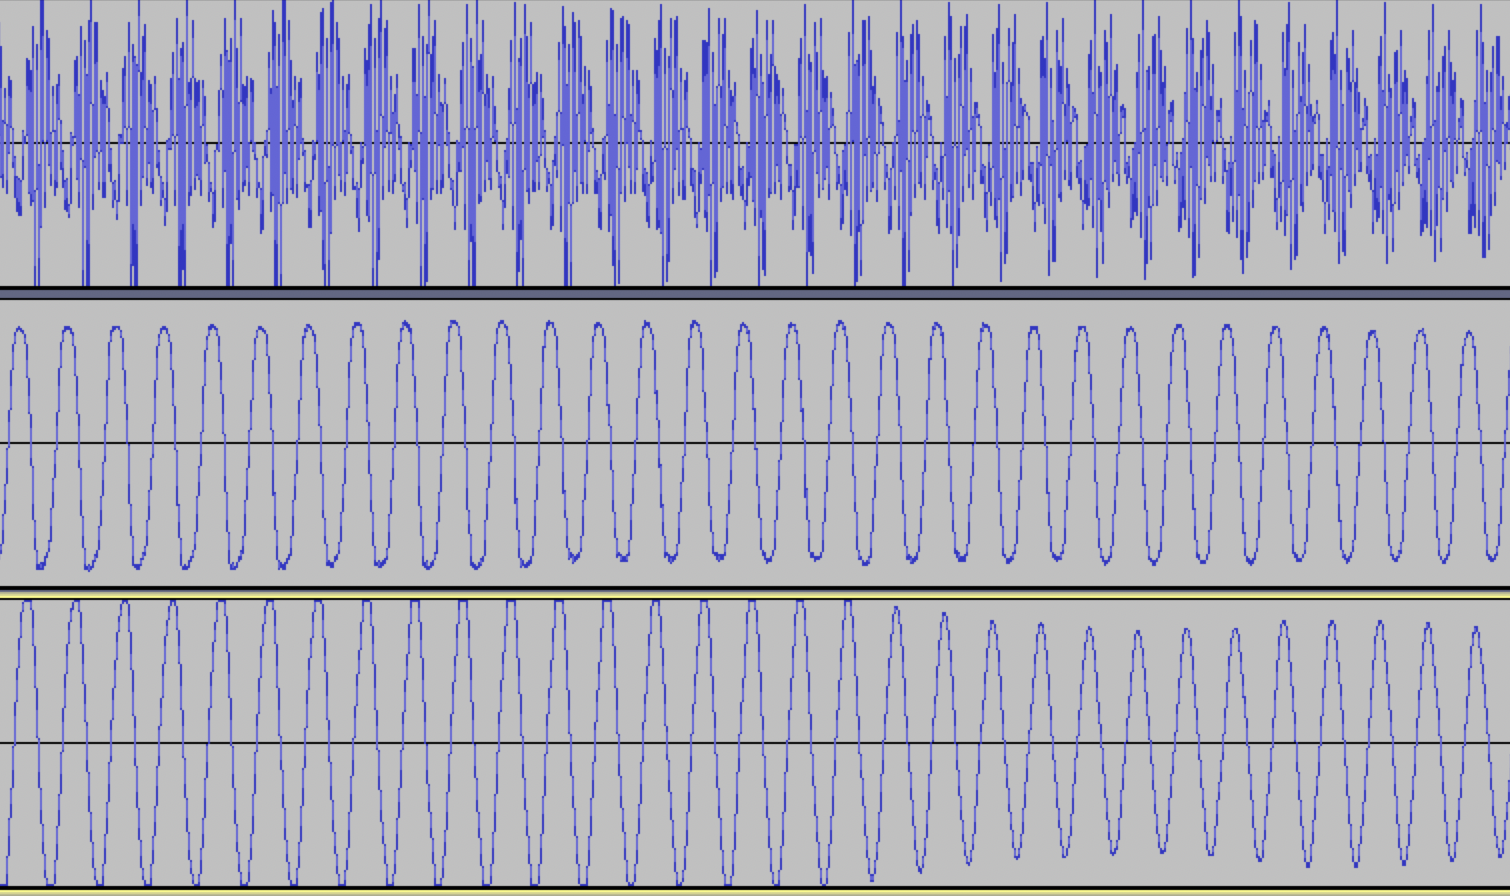
\includegraphics[width=0.7\hsize]{figure/66_22_det/d4s_0100_0200.png}
\caption{D4$\sharp$の0.100秒から0.200秒までの音波}
\label{fig:66_22_near}
\end{center}
\end{figure}

\ref{sec:expression}節と同程度にハープに近い音が生成される場合もあった。具体的には、D4,D4$\sharp$,G4,F5,F5$\sharp$の音である。これらの音は、音波が図\ref{fig:66_22_near}のように単純な波形でニューラルネットワークによる表現が容易であるため、生成が他の音波に比べて容易であったと考えられる。

\subsubsection{音波の複雑さ}

\begin{figure}[t]
\begin{center}
\begin{minipage}{0.48\hsize}
\begin{center}
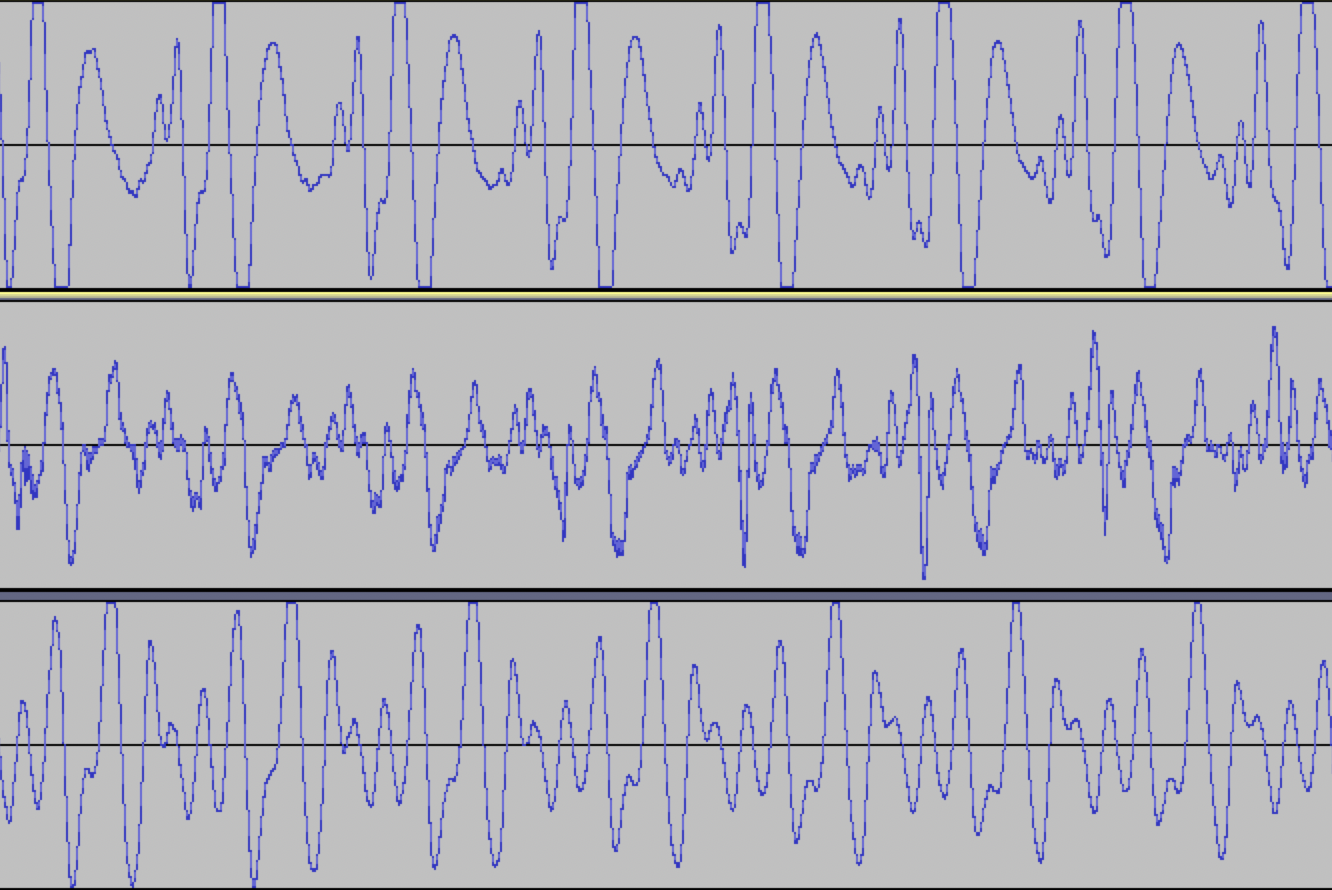
\includegraphics[width=0.9\hsize]{figure/66_22_det/d1_0300_0500.png}
\caption{D1の0.300秒から0.500秒までの音波}
\label{fig:66_22_bad1}
\end{center}
\end{minipage}
\begin{minipage}{0.48\hsize}
\begin{center}
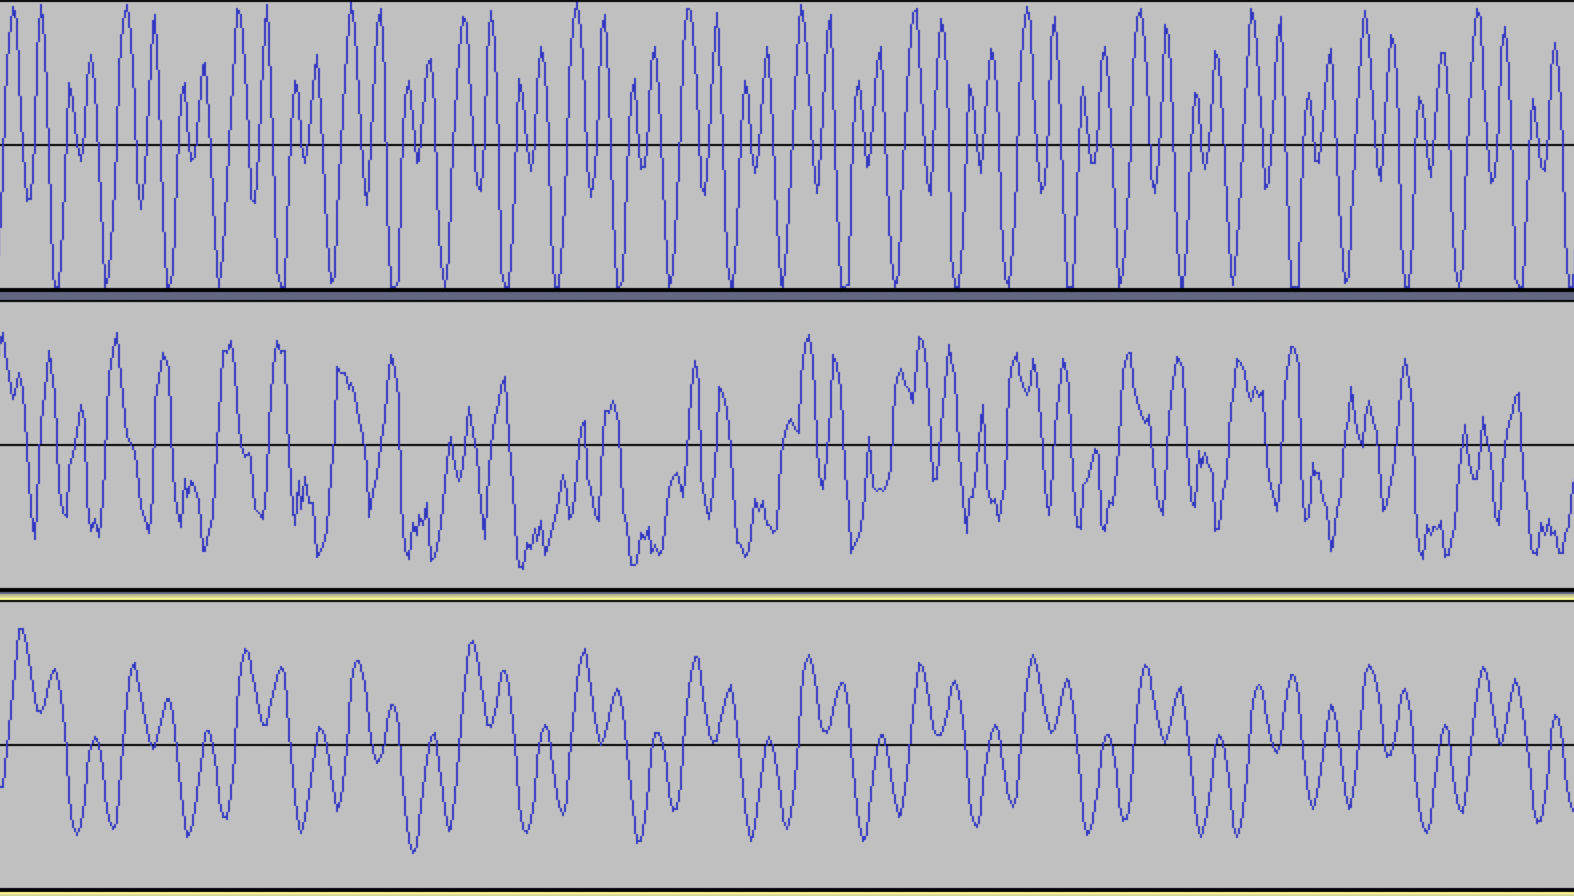
\includegraphics[width=0.9\hsize]{figure/66_22_det/f6_0070_0080.png}
\caption{F6の0.070秒から0.080秒までの音波}
\label{fig:66_22_bad2}
\end{center}
\end{minipage}
\end{center}
\end{figure}

\begin{figure}[t]
\begin{center}
\begin{minipage}{0.48\hsize}
\begin{center}
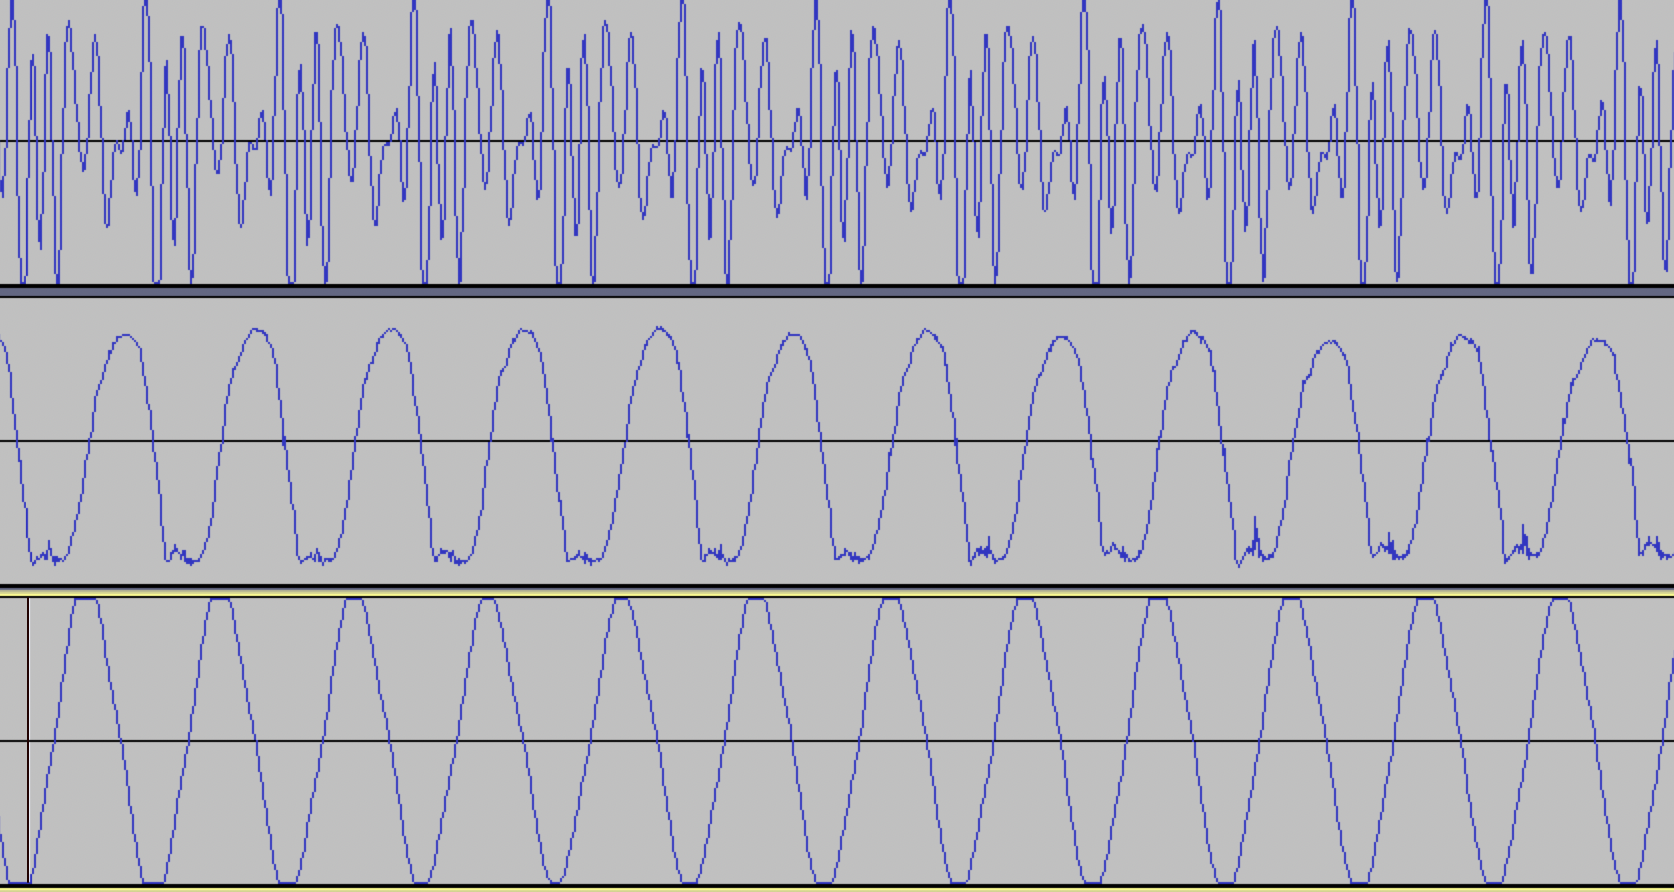
\includegraphics[width=0.9\hsize]{figure/66_22_det/g4s_0150_0180.png}
\caption{G4$\sharp$の0.150秒から0.180秒までの音波}
\label{fig:66_22_bad3}
\end{center}
\end{minipage}
\begin{minipage}{0.48\hsize}
\begin{center}
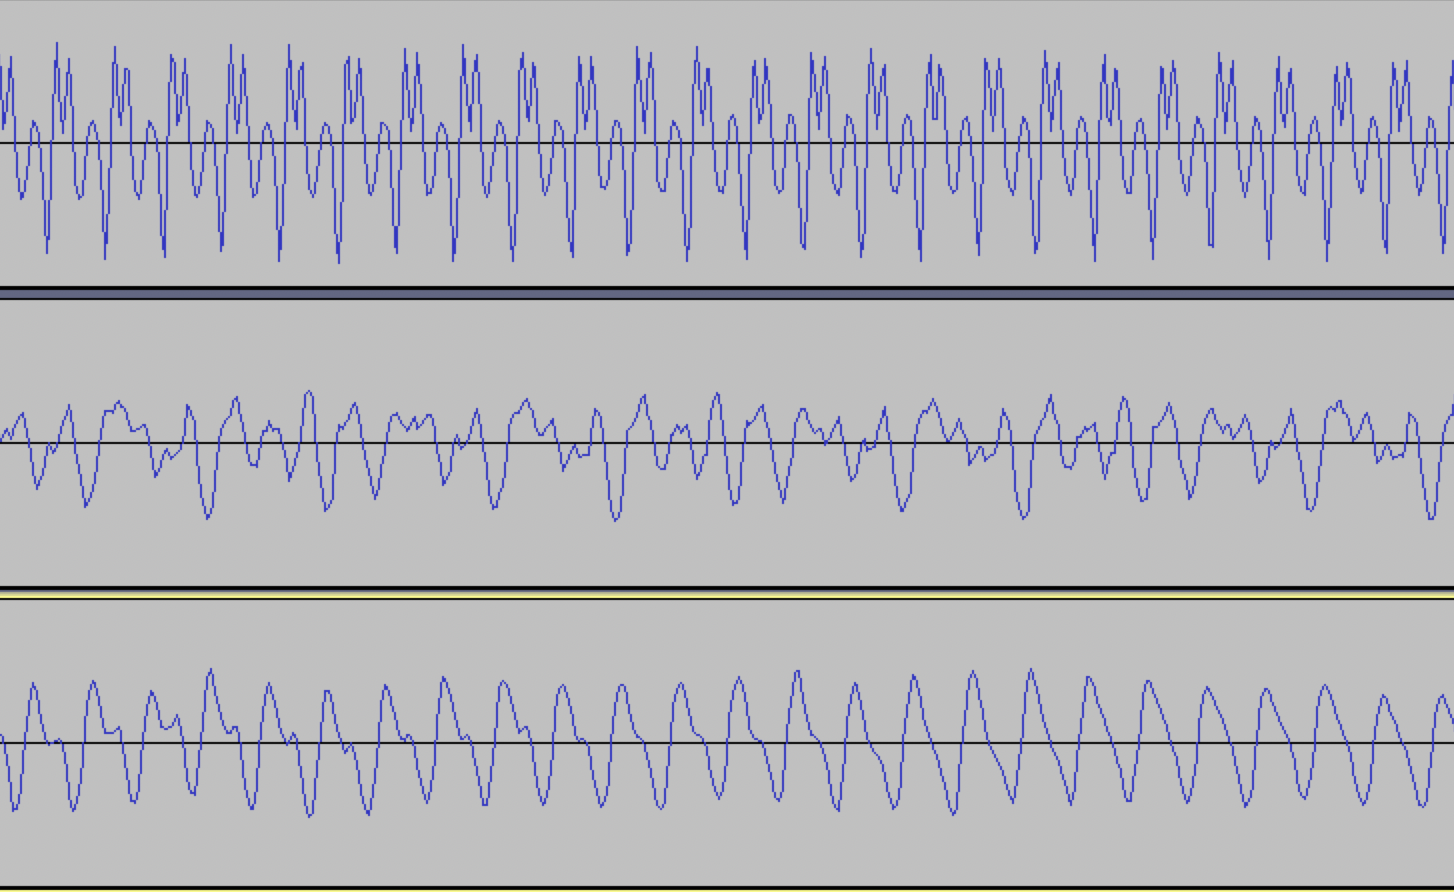
\includegraphics[width=0.9\hsize]{figure/66_22_det/d7s_0100_0110.png}
\caption{D7$\sharp$の0.1700秒から0.110秒までの音波}
\label{fig:66_22_bad4}
\end{center}
\end{minipage}
\end{center}
\end{figure}

上記の単純な音波以外の場合はギターの音色とは異なるもののハープの音色とも異なる音が生成された。いくつか種類があったが、図\ref{fig:66_22_bad1}や図\ref{fig:66_22_bad2}のように、音波が安定した振動をせず上音の成分がハープよりも多い音波が多く観測された。

また、ほとんどの音波において基音は保たれていたが、図\ref{fig:66_22_bad3}のように基音が同じで位相が異なる音波や図\ref{fig:66_22_bad4}のように基音が異なる音波が生成されることもあった。

これらの原因は、振幅をランダムにすることにより学習が安定しないことと微細な振動を表現可能なニューラルネットワークを構築できていないためと考えられる。後者の場合は画像で用いられるGANでの画像の高解像度化の工夫が適用できると期待される。